\documentclass{beamer}
\mode<presentation>
\usepackage{amsmath}
\usepackage{amssymb}
%\usepackage{advdate}
\usepackage{adjustbox}
\usepackage{subcaption}
\usepackage{enumitem}
\usepackage{multicol}
\usepackage{gensymb}
\usepackage{mathtools}
\usepackage{listings}
\usepackage{hyperref}
\usepackage{url}
\def\UrlBreaks{\do\/\do-}
\usetheme{Boadilla}
\usecolortheme{lily}
\setbeamertemplate{footline}
{
  \leavevmode%
  \hbox{%
  \begin{beamercolorbox}[wd=\paperwidth,ht=2ex,dp=1ex,right]{author in head/foot}%
    \insertframenumber{} / \inserttotalframenumber\hspace*{2ex} 
  \end{beamercolorbox}}%
  \vskip0pt%
}
\setbeamertemplate{navigation symbols}{}

\providecommand{\nCr}[2]{\,^{#1}C_{#2}} % nCr
\providecommand{\nPr}[2]{\,^{#1}P_{#2}} % nPr
\providecommand{\mbf}{\mathbf}
\providecommand{\pr}[1]{\ensuremath{\Pr\left(#1\right)}}
\providecommand{\qfunc}[1]{\ensuremath{Q\left(#1\right)}}
\providecommand{\sbrak}[1]{\ensuremath{{}\left[#1\right]}}
\providecommand{\lsbrak}[1]{\ensuremath{{}\left[#1\right.}}
\providecommand{\rsbrak}[1]{\ensuremath{{}\left.#1\right]}}
\providecommand{\brak}[1]{\ensuremath{\left(#1\right)}}
\providecommand{\lbrak}[1]{\ensuremath{\left(#1\right.}}
\providecommand{\rbrak}[1]{\ensuremath{\left.#1\right)}}
\providecommand{\cbrak}[1]{\ensuremath{\left\{#1\right\}}}
\providecommand{\lcbrak}[1]{\ensuremath{\left\{#1\right.}}
\providecommand{\rcbrak}[1]{\ensuremath{\left.#1\right\}}}
\theoremstyle{remark}
\newtheorem{rem}{Remark}
\newcommand{\sgn}{\mathop{\mathrm{sgn}}}
\providecommand{\abs}[1]{\left\vert#1\right\vert}
\providecommand{\res}[1]{\Res\displaylimits_{#1}} 
\providecommand{\norm}[1]{\lVert#1\rVert}
\providecommand{\mtx}[1]{\mathbf{#1}}
\providecommand{\mean}[1]{E\left[ #1 \right]}
\providecommand{\fourier}{\overset{\mathcal{F}}{ \rightleftharpoons}}
%\providecommand{\hilbert}{\overset{\mathcal{H}}{ \rightleftharpoons}}
\providecommand{\system}{\overset{\mathcal{H}}{ \longleftrightarrow}}
	%\newcommand{\solution}[2]{\textbf{Solution:}{#1}}
%\newcommand{\solution}{\noindent \textbf{Solution: }}
\providecommand{\dec}[2]{\ensuremath{\overset{#1}{\underset{#2}{\gtrless}}}}
\newcommand{\myvec}[1]{\ensuremath{\begin{pmatrix}#1\end{pmatrix}}}



\title{10.3.3.1.4}
\author{EE24BTECH11021 - Eshan Ray}
\date{\today}

\begin{document}

\begin{frame}
    \titlepage
\end{frame}

\begin{document}


\begin{frame}
    \frametitle{Problem Statement}
    Solve the following system of equations:
    \begin{align*}
        0.2x + 0.3y &= 1.3 \\
        0.4x + 0.5y &= 2.3
    \end{align*}
\end{frame}

\begin{frame}
    \frametitle{Method 1: Row Reduction}
    The following system of equations can be written in matrix form:-
\begin{align}
  Ax&= b  
\end{align}
where,
\begin{align}
    A &= \myvec{0.2&0.3\\0.4&0.5}\\
    b &= \myvec{1.3\\2.3}\\
    x &= \myvec{x\\y}\\
\end{align}
The augmented matrix $[A|b]$ is:
\begin{align}
    \myvec{0.2 & 0.3 &| 1.3\\0.4 & 0.5&|2.3}
    \end{align}
    \end{frame}
\begin{frame}
    \frametitle{Row Reduction Steps}
    Perform row operations:
    \begin{itemize}
        \item \( R_2 \rightarrow R_2 - 2R_1 \)
        \item \( R_1 \rightarrow R_1 + 3R_2 \)
        \item \( R_1 \rightarrow \frac{R_1}{0.2}, R_2 \rightarrow \frac{R_2}{-0.1} \)
    \end{itemize}
    Resulting augmented matrix:
    \begin{align}
        \myvec{1 & 0 & | 2 \\ 0 & 1 & | 3}
    \end{align}
    Thus, the solution is \( \brak{x, y} = \brak{2, 3} \).
\end{frame}

\begin{frame}
    \frametitle{Method 2: LU Decomposition}
    The matrix equation \( A \vec{x} = \vec{b} \) can be solved using LU Decomposition:
    \begin{align}
        A = LU
    \end{align}
    where \( L \) is a lower triangular matrix and \( U \) is an upper triangular matrix.
\end{frame}

\begin{frame}
    \frametitle{LU Decomposition - Step 1}
    Perform row reduction to decompose \( A \):
    \begin{align}
        \myvec{0.2 & 0.3 \\ 0.4 & 0.5} \xrightarrow{R_2 = R_2 - 2R_1} \myvec{0.2 & 0.3 \\ 0 & -0.1}
    \end{align}
    Let 
\begin{align}
    L = \myvec{1 & 0\\ l_{21} & 1}
\end{align}
$l_{21}$ is the multiplier used to zero $a_{21}$, so $l_{21} = 2$.\\
    The lower triangular matrix \( L \) is:
    \begin{align}
        L = \myvec{1 & 0 \\ 2 & 1}
    \end{align}
    And the upper triangular matrix \( U \) is:
    \begin{align}
        U = \myvec{0.2 & 0.3 \\ 0 & -0.1}
    \end{align}
\end{frame}
\begin{frame}
    \frametitle{Alternate LU Decomposition:DoLittle Algorithm}
    The LU Decomposition of matrix $A$ can also be obtained by Doolittle's Algorithm. This gives us update equations to construct the $L$ and $U$ matrix. \\
Elements of $U$ matrix:\\
For each column $j$,
\begin{align}
  U_{ij} = \begin{cases}
    A_{ij} & i=0 \\
    A_{ij} - \sum _{k=0}^{i-1} L_{ik}U_{kj} & i>0
  \end{cases}
\end{align}
Elements of $L$ matrix:\\
For each row $i$,
\begin{align}
  L_{ij} = \begin{cases}
    \frac{A_{ij}}{U_{ij}} & j=0 \\
    \frac{A_{ij} - \sum _{k=0}^{j-1} L_{ik}U_{kj}}{U_{ij}} & j>0
  \end{cases}
\end{align}
    
\end{frame}
\begin{frame}
    \frametitle{LU Decomposition - Step 2}
    Now solve the two systems:
    \begin{align}
        U \vec{x} &= \vec{y} \\
        L \vec{y} &= \vec{b}
    \end{align}
    First, solve \( L \vec{y} = \vec{b} \):
    \begin{align}
        \myvec{1 & 0 \\ 2 & 1} \myvec{y_1 \\ y_2} &= \myvec{1.3 \\ 2.3} \\
        \Rightarrow \vec{y} = \myvec{1.3 \\ -0.3}
    \end{align}
\end{frame}

\begin{frame}
    \frametitle{LU Decomposition - Step 3}
    Next, solve \( U \vec{x} = \vec{y} \):
    \begin{align}
        \myvec{0.2 & 0.3 \\ 0 & -0.1} \myvec{x_1 \\ x_2} &= \myvec{1.3 \\ -0.3} \\
        \Rightarrow \vec{x} = \myvec{2 \\ 3}
    \end{align}
    Thus, the point of intersection is \( \brak{2, 3} \).
\end{frame}

\begin{frame}
    \frametitle{Plot of the Solution}
    \begin{center}
        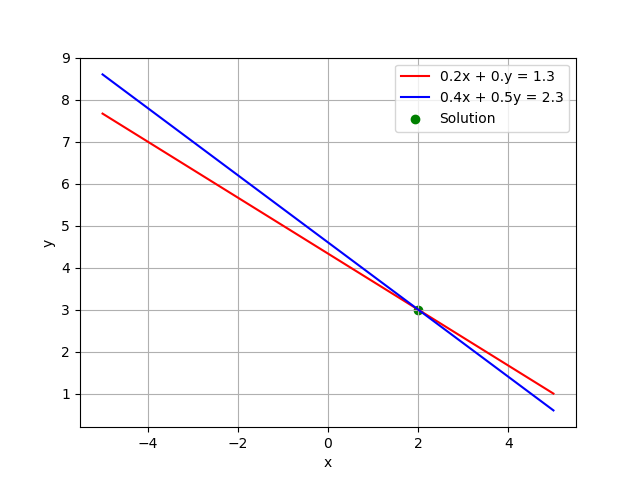
\includegraphics[width=0.7\textwidth]{plots/plot.png}
        \caption{Graphical Solution of the System of Equations}
    \end{center}
\end{frame}

\begin{frame}
    \frametitle{Conclusion}
    \begin{itemize}
        \item The system of equations was solved using two methods: Row Reduction and LU Decomposition.
        \item Both methods resulted in the solution \( \brak{2, 3} \), which is the point of intersection.
    \end{itemize}
\end{frame}
\begin{frame}
\frametitle{Codes}
    C code :\\
    \url{https://github.com/eshan810/ee1003/blob/main/Assignments/6/codes/code.c} \\
    Python code:\\
    \url{https://github.com/eshan810/ee1003/blob/main/Assignments/6/codes/plot.py} \\
 \end{frame}

\end{document}

